% 正方体 ABCD-A1B1C1D1 示意，E 为底面对角线交点，F 为侧面两对角线交点；虚线为遮挡棱与内部研究线段
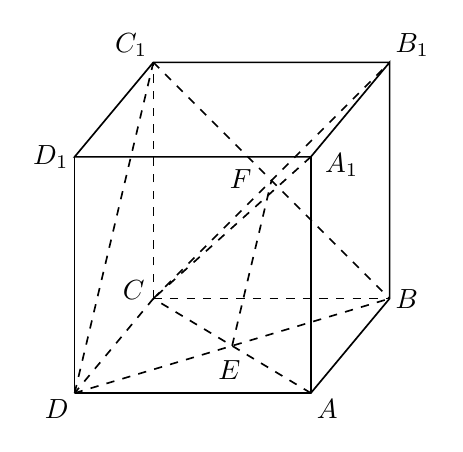
\begin{tikzpicture}[x=1cm,y=1cm,font=\normalsize,
  solidedge/.style={solid,line width=.6pt,draw=black},
  hidedge/.style={dashed,line width=.6pt,draw=black},
  ptlabel/.style={font=\normalsize,inner sep=2pt}]
\coordinate (D) at (0,0);
\coordinate (A) at (3,0);
\coordinate (C) at (1,1.2);
\coordinate (B) at (4,1.2);
\coordinate (D1) at (0,3);
\coordinate (A1) at (3,3);
\coordinate (C1) at (1,4.2);
\coordinate (B1) at (4,4.2);
\coordinate (E) at (2,0.6);
\coordinate (F) at (2.5,2.7);
% 可见轮廓
\draw[solidedge] (D) -- (A) -- (B) -- (B1) -- (A1) -- (D1) -- (C1) -- (B1);
\draw[solidedge] (D) -- (D1);
\draw[solidedge] (A) -- (A1);

% 遮挡棱（交于 C）
\draw[hidedge] (C) -- (B);
\draw[hidedge] (C) -- (D);
\draw[hidedge] (C) -- (C1);
% 底面对角线交于 E
\draw[hidedge] (D) -- (B);
\draw[hidedge] (A) -- (C);
% 侧面对角线交于 F
\draw[hidedge] (C1) -- (B);
\draw[hidedge] (C) -- (B1);
% 平面 BDC1 的边与垂线 A1C
\draw[hidedge] (D) -- (C1);
\draw[hidedge] (A1) -- (C);
% E-F 连线
\draw[hidedge] (E) -- (F);
\node[ptlabel,below left] at (D) {$D$};
\node[ptlabel,below right] at (A) {$A$};
\node[ptlabel,left,xshift=-1pt,yshift=3pt] at (C) {$C$};
\node[ptlabel,right] at (B) {$B$};
\node[ptlabel,left] at (D1) {$D_{1}$};
\node[ptlabel,right,xshift=3pt,yshift=-3pt] at (A1) {$A_{1}$};
\node[ptlabel,above left] at (C1) {$C_{1}$};
\node[ptlabel,above right] at (B1) {$B_{1}$};
\node[ptlabel,below,xshift=-1pt,yshift=-3pt] at (E) {$E$};
\node[ptlabel,above left,xshift=-5pt,yshift=-5pt] at (F) {$F$};
\end{tikzpicture}
